\section{Grundlagen}
\begin{frame}{}
    \begin{center}
        Grundlagen
     \end{center}
\end{frame}

\begin{frame}{Ein typisches Freifunk Netz}
    \begin{itemize}
        \item Ein Batman-Adv Netz
        \begin{itemize}
            \item[$\rightarrow$] "Wie ein großer dezentraler Switch"
        \end{itemize}
        \item VPN für die Funkinseln
        \begin{itemize}
            \item Multi-Client zu Multi-Client VPN
            \item Layer-II Netz
            \item Kein internes Routing / Forwarding
        \end{itemize}
        \item Mehrere VPN Server / Gateway
        \begin{itemize}
            \item DHCP
            \item DNS Namensauflösung
            \item Gateway zum Internet / ICVPN
        \end{itemize}
        \item Monitoring
        \begin{itemize}
            \item Karte aller Knoten
        \end{itemize}
    \end{itemize}
\end{frame}

\begin{frame}{Ein typisches Freifunk Netz}
    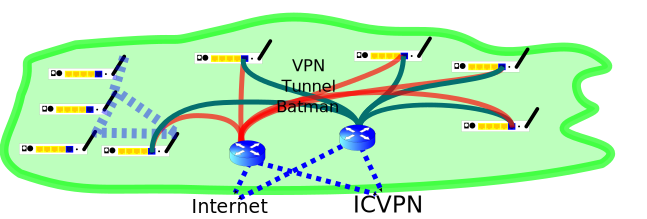
\includegraphics[width=\textwidth]{img/svg/freifunk_konzepte_alt.pdf}
\end{frame}

\begin{frame}{Freifunk Franken Netz}
    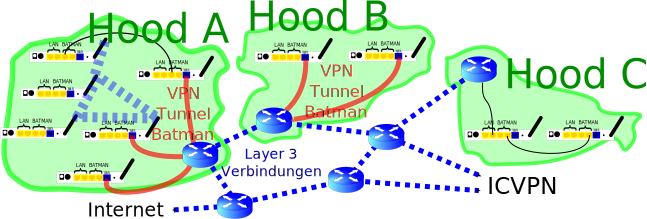
\includegraphics[width=\textwidth]{img/svg/freifunk_konzepte.pdf}

    \begin{itemize}
        \item Mehrere Layer-2 Inseln (Hoods)
        \item Verbindung per Layer-3
        \item Dezentrale Gateways
    \end{itemize}
\end{frame}
